\section {Introduction}

Many of the searches for \charginopm and \neutralinotwo in ATLAS and CMS involves the search for signal events with 3 leptons and \met. On the other hand there are very few searches involving final states with $\tau$ leptons due to the the larger $\tau$ misidentification rate which makes harder to keep the background under control as well as having low \pt thresholds for triggering.

There is however the possibility to study final states with $2\tau$ and \met coming from the decay of \charginopm and \neutralinotwo produced by Vector Boson Fusion (VBF) processes. This search comes with some important advantages.

Firstly with the increasing LHC luminosity both ATLAS and CMS needs to raise the \pt thresholds on the triggered objects. Is it possible however to probe signal for SUSY in VBF events by triggering over the VBF properties of the event, leaving the decay products of \charginopm and \neutralinotwo free from trigger bias. 

Secondly scenarios involving the naturalness of SUSY allows \stau lighter than \smuon and \selectron for high values of \tanbeta. A light \stau with small mass splitting also is favored in coannihilation processes \ref{cohannilation} that set the relic density to correct values, in the case of Bino dark matter. Light \stau is also motivated in the context of the MSSM by the enhancement of the $H \longrightarrow \gamma\gamma$ channel \ref{highsgammagamma}. All of these facts stress on the importance of the search for low \pt $\tau$ final states with large background contribution, for which production by the VBF processes since is possible to take advantage of its signature in order to reduce the background contribution to acceptable levels. 

As third and final reason a VBF based search can be complementary to the existing one at LHC based on Drell-Yan production since is not constrained by any trigger bias. 

\begin{figure}[tbh!]
	\centering
	\begin{tabular}{cc}
		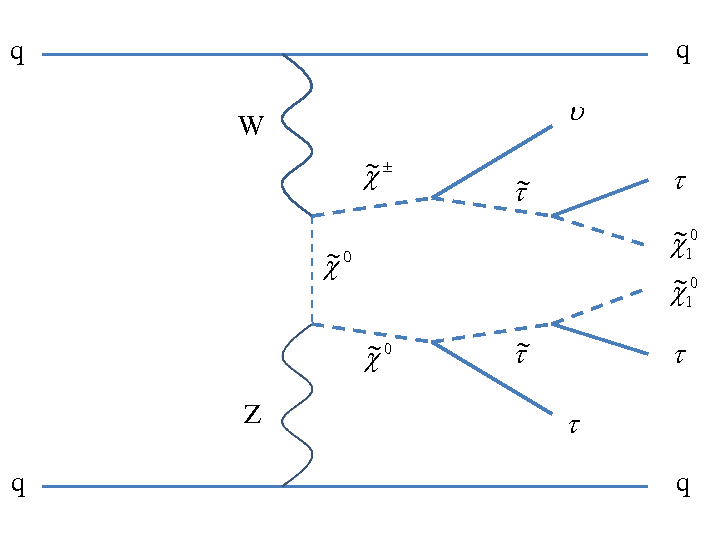
\includegraphics[width=0.50\textwidth]{analysis/pics/fig_FeynC1N2_Stau.png}
		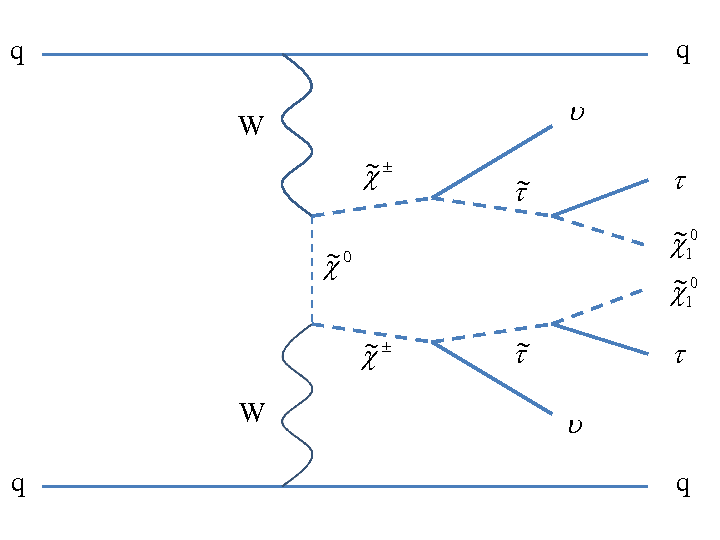
\includegraphics[width=0.50\textwidth]{analysis/pics/fig_FeynC1C1_Stau.png} 		
	\end{tabular}
	\caption{Diagrams of (left) \charginopm \neutralinotwo and (right) \charginopm \charginomp pair production through vector-boson fusion followed by their decays to $\tau$ leptons and the LSP.}
	\label{fig:VBF_diagrams}
\end{figure}

The Feynman diagrams for the typical \charginopm \neutralinotwo pair production are shown on  Figure \ref{fig:VBF_diagrams}. The \charginopm and \neutralinotwo coming from the VBF processes decays into the multiple leptons and \neutralinoone final state with the following decay process for \charginopm

\begin{equation}
\charginopm \longrightarrow \stau \nu \longrightarrow \neutralinoone \tau \nu
\end{equation}

and similarly for \neutralinotwo

\begin{equation}
\neutralinotwo \longrightarrow \stau \tau \longrightarrow \neutralinoone \tau \tau
\end{equation}

\section {Search Strategy}

For this type of search several benchmark points are defined under the following constraints:
\begin{itemize}
	\item The \charginopm and \neutralinotwo are mainly Wino, the \neutralinoone is mainly Bino;
	\item The \charginomp mass similar to the \neutralinotwo mass ($m_{\charginopm} \sim m_{\neutralinotwo}$) and with values of 100, 200 and 300 \gev;
	\item The mass gap between the \stau and \charginopm is either 5 \gev or $(m_{\stau} - m_{\charginopm})/2$;
	\item The LSP mass is either $\neutralinoone = 0 , 50 \gev$;
\end{itemize}

The processes taken into account are

\begin{equation}
pp \longrightarrow \charginopm \charginomp jj, \quad pp \longrightarrow \charginopm \neutralinotwo jj, \quad pp \longrightarrow \neutralinotwo \neutralinotwo
\end{equation}


The search strategy is based on two important steps: the first one is the reduction of the background contributions coming from V + jets events (where V is ether the W or Z boson) using the VBF properties of the event; the second is the usage of the properties of the centrally produces supersymmetric particles in order to reduce the all the non-supersymmetric background contributions.

The main feature of VBF processes is the production of two jets aimed at the forward-backward region of the detector with high \pt and large \deltaeta. By adding in the event selection the requirements on the di-jet \deltaeta as well as the di-jet invariant mass \ensuremath{m_{j_{1}j_{2}}} the background contribution coming from V+jets and \ttbar is kepts under control. 

(1) VBF processes: VBF processes are characterised by the production of two energetic jets produced in the forward-backward regions with large|∆η|. Requirements on |∆η| as well as Mj1j2, where Mj1j2 is the dijet invariant mass, are effective in reducing V +jets and tt background events, where the jets are less energetic and more central. Moreover, the leading jet is expected to have high pT since the incoming partons need significant momentum to create a pair of heavy supersymmetric states. This motivates a pT cut on the leading jet to reduce background.


